\chapter{Materály a metódy}

\section{Získanie bibliometrických dát}

\subsection{Celá fakulta}
\label{sec.all.mining}

Pre potreby tejto práce sme získali bibliografické údaje, ktorých aspoň jeden
z~autorov má príslušnosť (ang. \emph{affiliation}) k~FPV UCM v~Trnave. Na túto
analýzu sme nepoužili GS, pretože neumožňuje vyhľadávať podľa inštitúcie.

Bibligrafické záznamy FPV UCM sme získali z~citačných registrov WoS a Scopus dňa
21.\,decembra~2016.  Prístup k~obom citačným registrom bol umožnený
prostredníctvom webovej služby \emph{Centra Vedecko-Technických Informácií
  SR}\footnote{\url{http://www.cvtisr.sk}} (ďalej len CVTI SR).  Webové nástroje
Scopusu umožňujú vyhľadávať záznamy podľa inštitúcie (sekcia \emph{Affiliation
  search}).

Následne sme fitrovali publikácie, ktoré patria do FPV, pretože Scopus
neumožňuje zobraziť záznamy podľa príslušnosti k~fakulte danej inštitúcie.
Vyňali sme (\texttt{EXCLUDE}) publikácie podľa vedeckých oblastí
(\texttt{SUBJAREA}), ktoré nesúvisia s~činnosťou FPV:

\begin{itemize}
\item \emph{Art and Humanites} (\texttt{ARTS}): spoločenské a humanitné vedy,
\item \emph{Social Sciences} (\texttt{SOCI}): sociálne vedy,
\item \emph{Economics} (\texttt{ECON}): ekonómia,
\item \emph{Decision Science} (\texttt{DECI}): rozhodovacie vedy,
\end{itemize}
a časopisov (\texttt{EXACTSRCTITLE}), v~ktorých pracovníci FPV nepublikovali:

\begin{itemize}
\item \emph{Pediatrika},
\item \emph{Serbian Journal of Managment},
\item \emph{Wound Repair and Regeneration}.
\end{itemize}

Ďalej sme z~dát sme vypustili všetky publikácie prof. MUDr.\,Jozefa
Rovenského,\,DrSc.  (\texttt{AU-ID}: \uv{Rovenský, Jozef A.} a \uv{Rovenský,
  Jozef}), pretože je pracovníkom Inštitútu fyzioterapie, balneológie a
liečebnej rehabilitácie UCM. Tiež sme vyňali publikácie z~roku
(\texttt{PUBYEAR}) 1991, pretože v~tom období UCM ešte nebola založená, teda sme
to zhodnotili ako chybu v~databázi.

Výsledný vyhľadávací reťazec (Obrázok \ref{fig:scopus.query}), sme zadali (po
odstránení zalomenia riadku) do poľa \emph{search} na webových stránkach Scopus
a získali sme zoznam publikácií FPV UCM v~Trnave (obsahuje 360 záznamov). Ten
sme stiahli, pomocou fukncie \emph{Export all} (Označili sme formát
CSV\footnote{Formát textového súboru, ktorý obsahuje tabuľku dát. Jednotlivé
  riadky súboru zodpovedajú riadkom tabuľky a položky jednotlivých stĺpcoch sú
  oddelené čiarkou a prípadne ohraničené úvodzovkami.  Názov formátu pochádza
  z~ang.  \emph{comma-separated values}} a položku \emph{Citation information
  only} \footnote {Použitie iných možnosti bráni otvoreniu CSV súboru v~programe
  PoP \citep{Harzing2011}}).  Pretože exportovaný súbor zo Scopusu má iné
poradie položiek ako ten z~programu PoP, sme ešte súbor otvorili v~programe PoP
a v~ňom exportovali do formátu CSV.


\begin{figure}
  \footnotesize
  \begin{Verbatim}[frame=single]
    AF-ID ( "University of SS Cyril and Methodius Trnava"   60021677 )  AND
      ( EXCLUDE ( SUBJAREA ,  "ARTS" ) )  AND
      ( EXCLUDE ( PUBYEAR ,  1991 ) )  AND
      ( EXCLUDE ( SUBJAREA ,  "ECON" ) )  AND
      ( EXCLUDE ( SUBJAREA ,  "SOCI" ) )  AND
      ( EXCLUDE ( EXACTSRCTITLE ,  "Serbian Journal Of Management" ) )  AND
      ( EXCLUDE ( SUBJAREA ,  "DECI" ) )  AND
      ( EXCLUDE ( EXACTSRCTITLE ,  "Wound Repair And Regeneration" ) )  AND
      ( EXCLUDE ( AU-ID ,  "Rovenský, Jozef A."   55356120400 )  OR
      EXCLUDE ( AU-ID ,  "Rovenský, Jozef"   56351633900 ) )  AND
      ( EXCLUDE ( EXACTSRCTITLE ,  "Pediatrika" ) )
  \end{Verbatim}
  \vspace*{-4mm}
  \caption[Vyhľahávaci reťazec pre celú fakultu pre Scopus]%
  {Vyhľadávací reťazec pre Scopus na zobrazenie zoznamu všetkých publikácii FPV
    UCM v~Trnave.  Z~celej fakulty (\texttt{AF-ID}) sme vyčlenili
    (\texttt{EXCLUDE}) podľa vedeckých oblastí (\texttt{SUBJAREA}): spoločenské
    a humanitné vedy (\texttt{ARTS}), sociálne vedy (\texttt{SOCI}), ekonómia
    (\texttt{ECON}), rozhodovacie vedy (\texttt{DECI}) a časopisov
    (\texttt{EXACTSRCTITLE}).  Odstrálili sme práce prof. MUDr.\,Jozefa
    Rovenského,\,DrSc.  (\texttt{AU-ID}, ktorý pracuje na Inštitúte
    fyzioterapie, balneológie a liečebnej rehabilitácie a publikácie z~roku
    (\texttt{PUBYEAR}) 1991, kedy fakulta ešte nebola založená. Pre zadanie
    reťazca je nutné odstrániť zalomenia riadkov.}
  \label{fig:scopus.query}
\end{figure}


Na webové stránky WoS sme prispupovali cez portál CVTI SR. Nástroje WoS nám
neumožnili vyhľadávať podľa inštitúcie, ako v~nástroje Scopusu, preto sme boli
nútený hľadávať podľa adresy inštitúcie. Na webových stránkach WoS sme do poľa
pre hľadanie podľa adresy inštitúcie zadali: \uv{methodius*} a \uv{Trnava},
pretože v~publikáciách sa vyskytujú rôzne varianty názvu univerzity (napr. SS
Cyril \& Methodius Trnava, alebo Sv. Cyril and Methodius Trnava).  Aby sme
získali iba publikácie FPV, tak zoznam publikácií sme zúžili (použitím funkcie
\emph{Refine}) na záznamy z~vedy a techniky (\emph{SCIENCE TECHNOLOGY}) a
odstránili sme publikácie vedeckých oblastí mimo odborného záberu FPV:

\begin{itemize}
\item \emph{ORTHOPEDICS}: ortopédia,
\item \emph{PEDIATRICS}: pediatria,
\item \emph{RHEUMATOLOGY}: reumatológia,
\item \emph{SOCIAL SCIENCES OTHER TOPICS}: iné oblasti sociálnych vied,
\item \emph{SOCIOLOGY}: sociológia,
\item \emph{SURGERY}: chirurgia.
\end{itemize}

\begin{figure}
  \footnotesize
  \begin{Verbatim}[frame=single]
    ADDRESS: (methodius* AND Trnava) Refined by: RESEARCH DOMAINS:
      ( SCIENCE TECHNOLOGY ) AND [excluding] RESEARCH AREAS:
      ( SOCIOLOGY OR SURGERY OR SOCIAL SCIENCES OTHER TOPICS
      OR ORTHOPEDICS OR PEDIATRICS OR RHEUMATOLOGY )

    Timespan: 2000-2017.
    Search language=Auto
  \end{Verbatim}
  \vspace*{-4mm}
  \caption[Popis kritérií vyhľadávania vo WoS pre FPV]%
  {Popis vyhľadávacích krítérií, podľa ktorých sme vyhľadávali vo Web of Science
    všetky publikácie FPV UCM v~Trnave.  Hľadali sme podľa adresy inštitúcie
    (\texttt{ADDRESS}) so zameraním na vedu a technológiu (\texttt{SCIENCE
      TECHNOLOGY}) a vylúčili sme vybrané oblasti výskumu -- sociológiu,
    chirurgiu, iné oblasti sociálnych vied, ortopédiu, pediatriu, a
    reumatológiu.}
  \label{fig:wos.query}
\end{figure}


Počet výsledkov hľadania sme zúžili na 315 záznamov. Pre názornosť uvádzame
popis kritérií hľadania (Obrázok \ref{fig:wos.query}), ktorý je zobrazený na
webových stránkách WoS.  V~zozname sme našli 4 publikácie, ktoré nenapísali
pracovníci FPV.  Vyňatie prebeho tak, že pomocou funkcie \emph{Marked list} sme
označili všetky publikácie okrem:

\begin{itemize}
\item \emph{Left-handedness preferences, functions and dependence on neurotic
    behavior limited by specific social dimensions},
  % príslušnosť patrí katedre Psychológie, Filozofická fakulta UCM,
\item \emph{Intensification of menopausal symptoms among female inhabitants of
    East European countries},
  % príslušnosť patrí Inštitútu fyzioterapie, balneológie a liečebnej
  % rehabilitácie,
\item \emph{FAMILY CARE AS THE MOST SIGNIFICANT SYSTEM BARRIER TO WOMEN'S
    POLITICAL ACTIVITIES IN SLOVAKIA ON THE EXAMPLE OF MUNICIPAL FEMALE-MAYORS},
  % príslušnosť patrí Fakulte sociálnych vied UCM,
\item \emph{Treatment of lupus-nephritis and its course through the maintenance
    therapy},
  % príslušnosť patrí Inštitútu fyzioterapie, balneológie a liečebnej
  % rehabilitácie,
\end{itemize}

Následne sme zoznam publikácii uložený v~\emph{Marked list} stiahli ako textový
súbor s~použitím funkcie \emph{Save to Other Formats} (uložiť do iných formátov)
a v~okne \emph{Send to File} sme zvolili položku vo vyskakujúcom menu
\emph{Tab-delimited (Win, UTF-8)}. Na konverziu do formátu CSV je potrebné súbor
otvoriť v~programe PoP \citep{Harzing2011} a v~ňom ho exportovať vo~formáte CSV.


\subsection{Pracovníci fakulty}
\label{sec:staff.mining}

Na scientometrickú analýzu inštitúcie je vhodnejšie použiť bibliografické
informácie všetkých publikácií pracovníkov danej inštitúcie, nie len tých
publikácií, ktoré boli napísané v~rámci danej inštitúcie. Pretože ak vedecký
pracovník s~bohatou vyskumnou minulosťou nastúpi na nové pracovisko, prinesie zo
sebou skúsenosti a znalosti, čím zvýši kredit danej inštitúcie
\citep{Altanopoulou2012}.

Postupovali sme podľa prác \citet{Kazakis2014a} a
\citet{Kazakis2014b,Kazakis2015}.  Z~webových stránok FPV UCM v~Trnave
\footnote{\url{http://fpv.ucm.sk/sk/}} a webových stránok jednotlivých katedier
(Obrázok \ref{tab:department.review}) sme stiahli mená vedeckých pracovníkov FPV
UCM v~Trnave v~decembri 2016.

\begin{table}
  \centering\small
  \caption[Zoznam katedier FPV]%
  {Zoznam katedier FPV a ich oficiálných skratiek, s~odkazmi na webové stránky}
  \label{tab:department.review}
  \begin{tabularx}{\textwidth}{lll}
    \toprule
    Názov katedry & Skr. & Webová stránka \\
    \midrule
    Katedra biológie             & KB   & {\footnotesize \url{http://kb.fpv.ucm.sk/}}                       \\[0.5ex]
    Katedra biotechnológií       & KBt  & {\footnotesize \url{http://katedra-biotechnologii.webnode.sk/}}   \\[0.5ex]
    Katedra chémie               & KCh  & {\footnotesize \url{http://kchfpv.weebly.com/}}                   \\[0.5ex]
    Katedra ekochémie            & KER  & {\footnotesize \url{http://ker.fpv.ucm.sk/}}                      \\[-0.25ex]
    a rádiobiológie              &      &                                                                   \\ [0.5ex]
    Kat. aplikovanej informatiky & KAIM & {\footnotesize \url{http://ki.fpv.ucm.sk/}}                       \\[-0.25ex]
    a matematiky                 &      &                                                                   \\[0.5ex]
    Katedra biofyziky            & KBf  & {\footnotesize \url{http://fpv.ucm.sk/sk/katedra-biofyziky.html}} \\[0.5ex]
    Katedra odbornej jazykovej   & KOIP & {\footnotesize \url{http://kaj.fpv.ucm.sk/}}                      \\[-0.25ex]
    prípravy                     &      &                                                                   \\
    \bottomrule
  \end{tabularx}
\end{table}

\begin{table}
  \centering\small
  \caption[Rozdelenie pracovníkov do jednotlivých katedier]%
  {Rozdelenie pracovníkov, ktorých bibliometrické dáta sme použili v~tejto
    práci, do~jednotlivých katedier. Zoznam úplnych názvov katedier je
    uvedený v~Tabuľke \ref{tab:department.review}.}
  \label{tab:staff.list}
  \begin{tabularx}{\textwidth}{lll}
    \toprule
    Katedra & \multicolumn{2}{c}{Zoznam pracovníkov} \\
    \midrule
    KB   & prof. RNDr. Anna Preťová, DrSc.            & Mgr. Ľubica Uváčková, PhD.        \\
         & prof. RNDr. Juraj Krajčovič, CSc.          & RNDr. Zuzana Šramková, PhD.       \\
         & doc. Ing. Andrej Godány, CSc.              & RNDr. Lenka Tišáková, PhD.        \\
         & doc. Ing. Štefan Janeček, DrSc.            & RNDr. Barbora Vidová, PhD.        \\
         & doc. RNDr. Milan Seman, CSc.               & Mgr. Lenka Blažeková, PhD.        \\
         & doc. RNDr. Peter Siekel, CSc.              & Mgr. Lenka Raabová, PhD.          \\
         & Ing. Eva Ürgeová, PhD.                     &                                   \\[2ex]
    KBt  & prof. Ing. Stanislav Miertuš, DrSc.        & RNDr. Daniela Chmelová, PhD.      \\
         & prof. RNDr. Ján Kraic, PhD.                & Mgr. Daniel Mihálik, PhD.         \\
         & doc. RNDr. Miroslav Ondrejovič, PhD.       & Mgr. Katarína Lenghartová, PhD.   \\
         & doc. Ing. Stanislav Šilhár, CSc.           & RNDr. Jana Lomenová, PhD.         \\
         & doc. RNDr. Ján Rafay, CSc.                 & Ing. Tibor Maliar, PhD.           \\
         & RNDr. Michaela Havrlentová, PhD.           &                                   \\[2ex]
    KCh  & prof. Ing. Roman Boča, DrSc.               & doc. Ing. Ján Reguli, CSc.        \\
         & prof. Ing. Ernest Beinrohr, DrSc.          & Mgr. Peter Nemeček, PhD.          \\
         & prof. RNDr. Jaromír Pastorek, DrSc         & RNDr. Cyril Rajnák, PhD.          \\
         & prof. Ing. Oľga Križanová, DrSc.           & RNDr. Zita Tokárová, PhD.         \\
         & prof. Ing. Jozef Lehotay, DrSc.            & RNDr. Beáta Vranovičová, PhD.     \\
         & doc. Ing. Dušan Valigura, PhD.             & Ing. Jozef Miklovič, PhD.         \\
         & doc. Mgr. Renata Gašparová, PhD.           & Ing. Ján Rimarčík, PhD.           \\
         & doc. RNDr. Ján Titiš, PhD.                 & Ing. Mária Maliarová, PhD.        \\
         & doc. Ing. Jozef Sokol, CSc.                & Ing. Dáša Kružlicová, PhD.        \\[2ex]
    KER  & prof. Ing. Jozef Augustín, DrSc.           & Mgr. Ildikó Matušíková, PhD.      \\
         & doc. Dr. habil RNDr. Juraj Lesný, PhD.     & RNDr. Miroslav Horník, PhD.       \\
         & doc. Ing. Stanislav Hostin, PhD.           & RNDr. Anna Koprdová, PhD.         \\
         & doc. RNDr. Martin Pipíška, PhD.            &                                   \\[2ex]
    KAIM & prof. Ing. Vladimír Kvasnička, DrSc.       & PaedDr. Miroslav Ölvecký, PhD.    \\
         & prof. RNDr. Jiří Pospíchal, DrSc           & Ing. Miroslav Beňo, PhD.          \\
         & doc. RNDr. PaedDr. Ladislav Huraj, PhD.    & Ing. Darja Gabriška, PhD.         \\
         & doc. Ing. Michal Čerňanský, PhD.           & Ing. Jana Jurinová, PhD.          \\
         & doc. Ing. Branislav Hrúz, PhD.             & Ing. Marek Šimon, PhD.            \\
         & doc. Ing. German Michaľčonok, CSc.         & Ing. Andrea Vadkertiová, PhD.     \\
         & RNDr. Iveta Dirgová Luptáková, PhD.        & Mgr. Marián Hosťovecký, PhD.      \\
         & RNDr. Jaroslava Trubenová, PhD.            &                                   \\[2ex]
    KBf  & prof. Ing. Ivan Štich, DrSc.               & doc. RNDr. Ľubica Lacinová, DrSc. \\
         & doc. Mgr. Alžbeta Marček Chorvátová, DrSc. & RNDr. Júlia Horilová, PhD.        \\
         & doc. RNDr. Štefan Húšťava, PhD.            & Mgr. Michal Žitňan, PhD.          \\[2ex]
    KOJP & Mgr. Helena Zárubová                       & Mgr. Juraj Miština, PhD.          \\
    \bottomrule
  \end{tabularx}
\end{table}

Podľa Tabuľky \ref{tab:staff.list} sme vyhľadali záznamy jednotlivých
pracovníkov FPV z~citačných registrov Scopus, Web of Science a Google Scholar.
Dáta sú z~decembra 2016.

Databáza citačného register Scopus má špeciálnu indentitu pre autorov
(\texttt{AU-ID}).  Pomocou celého mena autora, priezviska, alebo jeho
príslušnosti (ang.  \emph{Affiliation}) je možné vyhľadať konkrétneho vedca a
získať iba jeho bibliometrické informácie. Niektorých prípadoch mal jeden
akademik niekoľko \texttt{AU-ID} (napr. Godány mal až tri). V~taktomto prípade
sme stiahli bibliografické záznamy všetkých identít do súborov vo formáte CSV a
súbory spojili do jedného súboru.  Vďaka \texttt{AU-ID} Scopus dokáže najsť
autora bezohľadu na to, či meno je zadané s~diakritikou, alebo nie.  Napriek
tomu sa vyskytli ľudia, ktorých Scopus nenašiel (viď Tabuľka
\ref{tab:staff.missing}).

WoS umožňuje vyhľadávať autorov len podľa priezviska a nemá taký prepracovaný
systém uloženej identity autora ako Scopus. Z~toho dôvodu, ak meno pracovníka
obsahuje diakritiku, tak sme v~rozšírenom výhľadávaní hľadali rôzne varianty
s~chýbajúcom diakritikou. Následne sme museli zoznam publikácie triediť podľa
iniciál, pretože väčšina publikácií neobsahuje celé mená autorov. V~prípade
vyskytu rôznych autorov s~rovnakým priezviskom a inicál sme museli zoznam
triediť podľa vednej oblasti. Nakoniec sme zoznam porovnali z~dátami zo Scopusu
toho istého autora a články, ktoré sa vyskytovali v~Scopuse, ale nie WoS sme
hľadali podľa nadpisu vo WoS. Všetky relevantné záznamy sme uložili do
\emph{Marked list} a uložili ako iný formát (funkcia \emph{Save to Other
  Formats}). Stiahnutý textový súbor sme otvorili v~programe PoP a v~ňom sme
exportovali do CSV formátu.

V~GS sme vyhľadávali priamo v~programe PoP. Vytvorili sme nový dopyt pre
vyhľadávanie v~GS (\emph{New Google Scholar Query}). Do poľa \emph{Authors} sme
zadali meno pracovníka a spustili sme vyhľadávania. Pretože program neumožňuje
zadať alternatívy mena ako WoS, urobili sme niekoľko hľadaní vždy s~inou
variantou mena (napr. s~diakritikou, bez diakritiky, s~krsným menom, inicálmi).
Ak sa meno bežne vyskytuje v~publikáciach (napr. Seman), PoP vyhľadal maximálne
1\,000 záznamov, pretože GS neumožnuje zobraziť viac výsledkov. Tak sme museli
vložiť do poľa \uv{všetký slová} (ang. \emph{All of the words}) reťazce, ktoré
bližšie určujú hľadané pracovníka ako napr.  \emph{Slovakia}.

Z~podstaty fungovania GS je zrejmé, že výsledný zoznam bude obsahovať veľa
balastu\footnote{Ako napr. záznamy iných autorov s~podobných, alebo rovnakým
  priezviskom a iniciálmi; záznamy, ktoré vôbec nesúvisia s~dopytom; duplicidné
  záznamy, nekopletné záznamy; nezmyselné záznamy.} (viď podapitola
\ref{sec:gs}).  Preto obsah CSV súboru z~PoP bolo potrebné ešte dodatočne
pretriediť a upraviť. Tento fakt uľahčovalo to, že väčšina záznamov obsahovala
internetový odkaz na zdroj. Ale aj tak bolo nutné doplniť chýbajúcich autorov
(GS ukazuje max 5 autorov) a roky.

Práce niektorých pracovníkov FPV sa nám vôbec nepodarilo vyhľadať. Príčinou bola
ich nedávna zmena mena po svadbe (viď Tabuľka \ref{tab:staff.rename} Našťastie
pôvodné priezivsko sme dohľadali z~akademickej emailovej adresy, ktorá bola
uverejnená na internetových stránkach katedry.

\begin{SCtable}
  \centering\small
  \caption[Mená pracovníkov FPV, u~ktorých došlo k~zmene priezivska]%
  {Zoznam pracovníkov FPV, u~ktorých došlo k~zmene priezivska. Pôvodné
    priezivsko sme dohľadali z~akademickej emailovej adresy.}
  \label{tab:staff.rename}
  \begin{tabular}{ll}
    \toprule
    Súčasné meno & Pôvodné meno \\
    \midrule
    Jana Lomenová & Jana Viskupičová \\
    Zita Tokárová & Zita Puterová    \\
    Anna Koprdová & Anna Sunovská    \\
    \bottomrule
  \end{tabular}
\end{SCtable}

\begin{SCtable}
  \centering\small
  \caption[Mená pracovníkov FPV, pre ktorých sa nám nepodarilo získať všetky
  dáta]%
  {Zoznam Pracovníkov FPV, pre ktorých sa nepodarilo získať z~niektorých
    citačných registrov žiadne dáta.  V~posledných troch sĺpcoch je uvedený
    počet publikácií, ktoré sa nám podarilo získať.}
  \label{tab:staff.missing}
  \begin{tabular}{lcccc}
    \toprule
    Meno pracovníka & Katedra & Scopus & WoS$^\dagger$ & GS$^\ddagger$ \\
    \midrule
    Lenka Raabová           &  KB  & 1  & --  & 3  \\
    Miroslav Beňo           & KAIM & -- & --  & 3  \\
    Jana Jurinová           & KAIM & -- & 2   & 11 \\
    Iveta Dirgová Luptáková & KAIM & 1  & --  & 6  \\
    Jaroslava Trubenová     & KAIM & -- & 3   & 6  \\
    Andrea Vadkertiová      & KAIM & -- & 1   & 6  \\
    \bottomrule \\[-2ex]
    \multicolumn{5}{l}{\footnotesize $^\dagger$ Web of Science; $^\ddagger$ Google Scholar}
  \end{tabular}
\end{SCtable}


\subsection{Zoznam časopisov}
\label{sec:journal.mining}

Obsahom tejto práce je hodnotenie fakulty na základe časopisov, v~ktorých jej
publikujú jej pracovníci. Vedecké časopisy je možné hodnotiť na základe
citačných indikátorov (viď Tabuľka \ref{tab:indicators.review}). Toto hodnotenie
vykonávajú medzinárodné ištitúcie (ako ISI, alebo SciMago) pre spektrum
svetových a domácich časopisov.

Zistili sme hodnoty impakt faktoru (viď podkapitola \ref{sec:if}, SciMago rang
časopisu, (viď podkapitola \ref{sec:sjr}), CiteScore (viď podkapitola
\ref{sec:citescore}) SNIP (viď podkapitola \ref{sec:snip}) pre všetky časopisy
z~bibliografických záznamov, ktorých proces získavania popisujeme v~podkapitole
\ref{sec.all.mining}.  Hodnoty pre IF sme získali z~oficiálnych internetových
stránok (viď Tabuľka \ref{tab:indicators.web}).  Zoznam časopisov je uvedený
v~Prílohe.  V~prípade ak citačný indikátor pre daný časopis sa nám nepodarilo
vyhľadať, tak sme položku v~zozname označili pomlčkou.

\begin{SCtable}
  \centering\small
  \caption[Webové stránky citačných indikátorov na hodnotenie časopisov]%
  {Zoznam citačných indikátorov na hodnotenie časopisov, s~odkazmi na oficiálne
    webové stránky}
  \label{tab:indicators.web}
  \begin{tabular}{ll}
    \toprule
    Názov citačného indikátoru      & Webová stránka\\
    \midrule
    impakt faktor         & {\footnotesize \url{http://www.scijournal.org}}         \\
    SciMago rang časopisu & {\footnotesize \url{http://www.scimagojr.com}}          \\
    CiteScore             & {\footnotesize \url{https://journalmetrics.scopus.com}} \\
    SNIP                  & {\footnotesize \url{http://www.scimagojr.com}}          \\
    \bottomrule
  \end{tabular}
\end{SCtable}

\section{Spracovanie bibliometrických dát}

\subsection{Program \emph{Publish or Perish}}
\label{sec:pop}

Na výpočet citačných indexov sme použili program \emph{Publish or Perish} verzie
5.25.2.6208 \citep{Harzing2011}.  PoP je voľne dostupná aplikácia pre operačný
systém Microsoft Windows na scientometrickú analýzu bibliografických záznamov.
Prirodzene umožňuje získavanie bibliografických záznamov z~GS a Microsoft
Academic. Prístup do GS je zdarma, ale pre prístup do MS Academic je potrebné
vložiť kľúč.  Ďalej umožňuje importovať a exportovať dáta do najrôznejších
formátov ako napr.  CSV, MS Exel, EndNote\footnote{\url{http://endnote.com/}}, a
BibTex\footnote{\url{http://www.bibtex.org/}}.  PoP umožňuje scienometrickú
analýzu s~použítím širokého spektra citačných indikátorov (časť, ktorú sme
použili v~tejto práci je uvedená v~Tabuľke \ref{tab:indicators.review}).  Súbor
dát, z~ktorého sa počítajú všetky indikátory sa nazýva dopyt
(ang. \emph{query}).  PoP neumožňuje editovať položky v~danom dopyte. Aby sme
mohli upraviť dáta, exportovali sme ich do~formátu CSV a editovali sme ich
v~externom programe.

Okno programu (viz Obrázok \ref{fig:pop.screenshot}) pozostáva z~troch rámcov:
\begin{itemize}
\item tabuľka dopytov s~vypočítanými indikátormi v~stĺpcoch,
\item tabuľka bibliografických záznamov v~označenom dopyte,
\item priečinkový strom na triedenie dopytov.
\end{itemize}

\begin{figure}
  \centering
  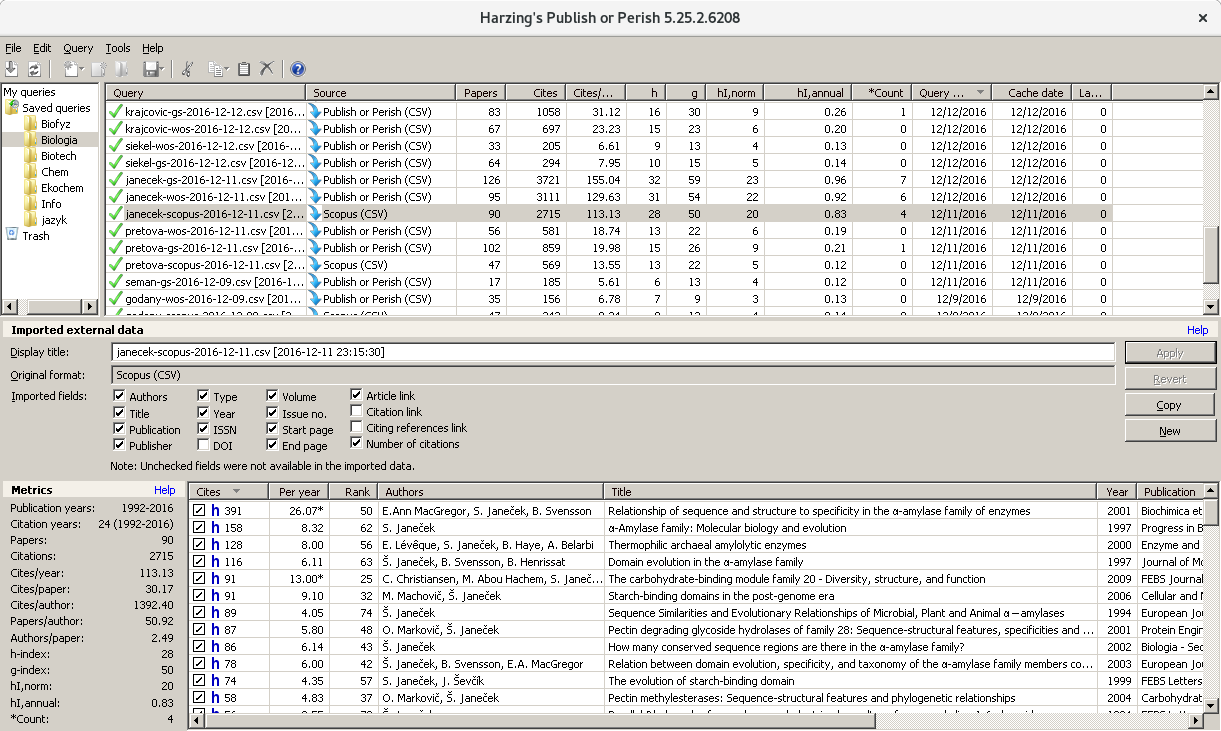
\includegraphics[width=\textwidth]{publish-or-perish_wine.png}
  \caption[Snímok obrazovky s~oknom programu \emph{Publish or Perish}.]%
  {Snímok obrazovky s~oknom programu \emph{Publish or Perish} (skrátene PoP),
    ktorý sme v~tejto práci použili na scientometrickú analýzu.  Ukážka
    zobrazuje scientometrické dáta jednotlivých pracovníkov FPV UCM
    v~Trnave. V~hornom rámci vidíme tabuľku pracovníkov s~citačnými
    indikátormi. V~dolnom rámci je zoznam publikácií označeného pracovníka. Na
    ľavej strane vidíme priečinkový strom, v~ktorom sú uložené dáta.}
  \label{fig:pop.screenshot}
\end{figure}


\subsection{Scientometrická analýza}

Podľa metodiky \citet{Kazakis2014a} a \citet{Kazakis2014b,Kazakis2015} sme
získali bibliografické údaje všetkých publikácií pracovníkov FPV a uložili sme
ich do CSV súborov. Tieto súbory sme importovali do PoP, kde sme zistili citačné
indikátory pre každého pracovníka. Vypočítané citačné indikátory dopytov
všetkých pracovníkov sme uložili do súborov s~názvami katedier, do ktorých
patria. Z~týchto súborov sme vybrali stĺpce, ktoré reprezentujú citačné
indikátory podľa Tabuľky \ref{tab:indicators.review} plus počet publikácií na
autora, počet citácií na publikáciu.  Záznamy sme usporiadali do skupín podľa
citačného registru, z~ktorého boli získané.  Vypočítali sme priemer, medián,
štandardnú odchýlku a MAD\footnote{Absolútna odchýlka mediánu
  (ang.\,\emph{Median Absolute Deviation}) je robustná štatistická metóda na
  zistenie rozptylu dát.  $\mathrm{MAD} = \mathrm{Med}(|X_i - \tilde{X}|)$.
  Keďže MAD využíva medián, je menej náchylný na extrémne vybočujúce hodnoty, a
  preto sa používa v~ distribúciách, ktoré sa príliš odchyľujú od normálnej
  distribúcie.\\\url{http://www.statisticshowto.com/median-absolute-deviation/}}
(absolútnu odchýlku mediánu) pre každú skupinu. Pre hodnoty počtu citácií a
publikácií sme nepočítali priemer a medián, ale sme spočítali sumu počtu citácii
a sumu počtu publikácii pre každú skupinu.

Nakoniec sme vytvorili dátový súbor s~18 riadkami (dáta zo Scopus, WoW a GS pre
každú katedru), ktorého každý riadok obsahuje skratku katedry a spracované dáta
jednotlivých citačných indikátorov.  Tieto dáta sme skonvertovali do Tabuliek
\ref{tab:1-staff.results}, \ref{tab:2-staff.results}, \ref{tab:3-staff.results},
\ref{tab:4-staff.results}, \ref{tab:5-staff.results} a
\ref{tab:6-staff.results}, ktore nájdeme v~nasledújúcej kapitole. Grafické
znázornenie sme vytvorili pomocou vlastného programu
\emph{scientometry-plot-gen} (viď podkapitola \ref{sec:program.my})

Na zhotovenie grafického znázornenia vývoja publikačnej a čitačnej činnosti FPV
sme použli bibliometrické dáta z~celej fakulty, ktorých získanie popisujeme
v~podkapitole \ref{sec.all.mining}. Z~jednotlivých dátových súborov (Scopus a
Wos) sme zistili počet publikácií na každý rok a celkovú sumu citácií na tieto
publikácie, tiež rozdelých podľa rokov. Na tento výpočet sme použili vlastný
progam \emph{scientometry-data-proc} (viď podkapitola \ref{sec:program.my}).

Z~bibliografických dát celej fakulty (proces získavania je popísaný
v~podkapitole \ref{sec.all.mining}) sme zistili koľko článkov bolo publikovaných
v~každom časopise.  Na túto úlohu sme použili vlastný progam
\emph{scientometry-data-proc}. Z~výstupu programu sme vytvorili časopisov
s~počtom výskytov publikácií a citačnými indikátormi príslušného časopisu (viď
Príloha)

\subsection{Vlastné programy na spracovanie a vizualizáciu dát}
\label{sec:program.my}

Pre účely tejto práce sme napísali programy \emph{scientometry-data-proc} na
spracovanie dát a \emph{scientometry-plot-gen} na vykreslenie grafov.  Obidva
programy sú napísané v~programovacom jazyku
Python\footnote{\url{https://www.python.org/}}. verzie 2.7.  Program
\emph{scientometry-plot-gen} využíva knižnicu \emph{matplotlib} na kreslenie
grafov.

Program \emph{scientometry-data-proc} sa konfiguruje pomocou štrukturovaného
textového súboru vo formáte YAML\footnote{\url{http://yaml.org/}} (viď
Príloha). Súbor, v~ktorom sú definované metadáta pre vykresľovanie grafov
pomocou programu \emph{scientometry-plot-gen} je tiež vo formáte YAML (v~Prílohe
sú oba súbory podrobne rozpísané).


%%% Local Variables:
%%% TeX-master: "diplomovka"
%%% End:
